\documentclass[a4paper,11pt]{article}

\usepackage[a4paper,left=2.5cm,right=2.5cm,top=3.5cm,bottom=3.5cm]{geometry}
\usepackage[utf8]{inputenc}
\usepackage[T1]{fontenc}
\usepackage[english]{babel}
\usepackage{graphicx}
\usepackage{amsmath,amssymb,amsthm,amsopn}
\usepackage{mathrsfs}
\usepackage{graphicx}
\usepackage{array}
\usepackage{makecell}
\usepackage{bm}
\usepackage{hyperref}
\usepackage[shortlabels]{enumitem}
\hypersetup{
    colorlinks=true,
    linkcolor=blue,
    citecolor=red,
}
\usepackage{diagbox}

\usepackage{algorithm}
\usepackage{algpseudocode}

\renewcommand{\algorithmicrequire}{\textbf{Input:}}
\renewcommand{\algorithmicensure}{\textbf{Output:}}

%\usepackage[top=1cm,bottom=1cm]{geometry}
%\usepackage{listings}
%\usepackage{xcolor}

\usepackage{tikz}
\usetikzlibrary{arrows}

% Tikz style

\tikzset{round/.style={circle, draw=black, very thick, scale = 0.7}}
\tikzset{arrow/.style={->, >=latex}}
\tikzset{dashed-arrow/.style={->, >=latex, dashed}}

\newtheoremstyle{break}%
{}{}%
{\itshape}{}%
{\bfseries}{}%  % Note that final punctuation is omitted.
{\newline}{}

\newtheoremstyle{sc}%
{}{}%
{}{}%
{\scshape}{}%  % Note that final punctuation is omitted.
{\newline}{}

\theoremstyle{break}
\newtheorem{thm}{Theorem}[section]
\newtheorem{lm}[thm]{Lemma}
\newtheorem{prop}[thm]{Proposition}
\newtheorem{cor}[thm]{Corollary}

\theoremstyle{sc}
\newtheorem{exo}{Exercice}

\theoremstyle{definition}
\newtheorem{defi}[thm]{Definition}
\newtheorem{ex}[thm]{Example}

\theoremstyle{remark}
\newtheorem{rem}[thm]{Remark}

% Math Operators

\DeclareMathOperator{\Card}{Card}
\DeclareMathOperator{\Gal}{Gal}
\DeclareMathOperator{\Id}{Id}
\DeclareMathOperator{\Img}{Im}
\DeclareMathOperator{\Ker}{Ker}
\DeclareMathOperator{\Minpoly}{Minpoly}
\DeclareMathOperator{\Mod}{mod}
\DeclareMathOperator{\Ord}{Ord}
\DeclareMathOperator{\ppcm}{ppcm}
\DeclareMathOperator{\tr}{Tr}
\DeclareMathOperator{\Vect}{Vect}
\DeclareMathOperator{\Span}{Span}
\DeclareMathOperator{\rank}{rank}
\DeclareMathOperator{\ev}{ev}

% Shortcuts

\newcommand{\dE}{\partial(E)}
\newcommand{\dF}{\partial(F)}
\newcommand{\dG}{\partial(G)}
\newcommand{\diff}{\mathop{}\!\mathrm{d}}
\newcommand{\eg}{\emph{e.g. }}
\newcommand{\emb}{\hookrightarrow}
\newcommand{\embed}[2]{\phi_{#1\hookrightarrow#2}}
\newcommand{\ent}[2]{[\![#1,#2]\!]}
\newcommand{\ie}{\emph{i.e. }}
\newcommand{\ps}[2]{\left\langle#1,#2\right\rangle}
\newcommand{\eqdef}{\overset{\text{def}}{=}}
\newcommand{\f}{f}%{\mathfrak{f}}
\newcommand{\bff}{\mathbf{f}}
\newcommand{\E}{\mathcal{E}}
\newcommand{\A}{\mathcal{A}}
\newcommand{\B}{\mathcal{B}}
\newcommand{\R}{\mathcal{R}}
\newcommand{\bfa}{\mathbf{a}}
\newcommand{\bfb}{\mathbf{b}}
\newcommand{\D}{\mathcal{D}}
\newcommand{\Pcal}{\mathcal{P}}
\newcommand{\musym}{\mu^{\textrm{sym}}}
\newcommand{\mutri}{\mu^{\textrm{tri}}}
\newcommand{\muhyp}{\mu^{\textrm{hyp}}}
\newcommand{\musymG}[1][G]{\mu^{\textrm{sym},#1}}
\newcommand{\mutriG}[1][G]{\mu^{\textrm{tri},#1}}
\newcommand{\muhypG}[1][G]{\mu^{\textrm{hyp},#1}}
\newcommand{\hmusym}{\hat\mu^{\textrm{sym}}}
\newcommand{\hmutri}{\hat\mu^{\textrm{tri}}}
\newcommand{\hmuhyp}{\hat\mu^{\textrm{hyp}}}
\newcommand{\hmusymG}[1][G]{\hat\mu^{\textrm{sym},#1}}
\newcommand{\hmutriG}[1][G]{\hat\mu^{\textrm{tri},#1}}
\newcommand{\hmuhypG}[1][G]{\hat\mu^{\textrm{hyp},#1}}
\newcommand{\Msym}{M^{\textrm{sym}}}
\newcommand{\Mtri}{M^{\textrm{tri}}}
\newcommand{\Mhyp}{M^{\textrm{hyp}}}
\newcommand{\hMsym}{\hat{M}^{\textrm{sym}}}
\newcommand{\hMtri}{\hat{M}^{\textrm{tri}}}
\newcommand{\hMhyp}{\hat{M}^{\textrm{hyp}}}
\newcommand{\tri}[2]{\mu_{#1}^{\text{tri}}(#2)}
\newcommand{\sym}[2]{\mu_{#1}^{m_3}(#2)}
\newcommand{\K}{\mathbf{k}}


% opening
\title{Tri-symmetric decompositions in finite fields}
\author{}



\begin{document}

\maketitle

\begin{abstract}
  To be written.
\end{abstract}

%\tableofcontents
%\clearpage

\section{Introduction}
\label{sec:intro}

\paragraph{Bilinear complexity.} Let $\K=\mathbb{F}_{q}$ be a finite field with
$q$ elements and $\A$
an algebra over $\K$. Given an algorithm dealing with elements in $\A$, one is
usually interested in the (asymptotic) cost of the algorithm. In order to
understand this cost, one studies the \emph{complexity} of the algorithm, \ie
the number of operations needed by the algorithm. We can for example count the number
of bit operations or the algebraic operations $(+, \times, \cdot)$ in the algebra
$\A$ or in the field $\K$. The latter is called the \emph{algebraic complexity}
and in this model we suppose that all algebraic operations have the same cost.
Nevertheless, multiplications in an algebra $\A$ are arguably more expensive than
additions or scalar multiplications. In the context of the computation of
bilinear maps, extensive work has been done to reduce the number of
multiplications involved. Notable examples are Karatsuba's
algorithm~\cite{Karatsuba63} and
Strassen's algorithm~\cite{Strassen69}. Karatsuba's algorithm is
based on the fact that the bilinear map associated to the product of two
polynomials of degree $1$
\[
  A = a_1 X + a_0\text{ and }B = b_1 X + b_0
\]
can be computed with three products $a_0b_0, (a_0+a_1)(b_0+b_1), a_1b_1$ instead
of the four classic ones $a_0b_0, a_0b_1, a_1b_0, a_1b_1$. Strassen's algorithm
exploits a similar idea in the case of $2\times2$ matrices: only $7$ products
are used instead of $8$ in order to compute a matrix product. Both these
algorithms have very practical consequences. The \emph{bilinear complexity}
$\mu(\A/\K)$ of the algebra $\A$ represents the minimum number of two-variable
multiplications in $\K$ needed to compute a product in $\A$, assuming that other
operations such as addition or multiplication by a constant have no cost. The
bilinear complexity is defined as the minimal number $n$ such that there exist
linear forms $(\varphi_i)_{1\leq i \leq n}$, $(\psi_i)_{1\leq i \leq n}$ in
$\A^\vee$, where $\A^\vee$ is the dual of $\A$, and
elements $(a_i)_{1\leq i \leq n}$ in $\A$ such that
\begin{equation}
  \forall x, y\in\A,\,xy = \sum_{i=1}^{n}\varphi_i(x)\psi_i(y)a_i.
  \label{eq:no-sym}
\end{equation}
Equivalently, it can be defined as the rank of the tensor in
\[
  \A^\vee \times \A^\vee\times \A
\]
corresponding to the multiplication map in $\A$. Let $\K^{2\times2}$ be the space
of $2\times2$ matrices over $\K$. We know thanks to Strassen's algorithm that 
\[
  \mu(\K^{2\times 2}/\K) \leq 7.
\]
In fact, this is optimal, so we have exactly $\mu(\K^{2\times2}/\K)=7$. In
general, it seems to be hard to find the bilinear complexity of a given algebra,
for example the bilinear complexity of $\K^{3\times3}$ is not known.
In the litterature, work has been done both to algorithmically find the bilinear complexity of
small algebras~\cite{BDEZ12, Covanov19} and to understand how the bilinear
complexity asymptotically grows~\cite{CC88, BCPRRR19}. Chudnovsky and Chudnosky
proved in 1988 that the bilinear complexity of an extension field
$\mathbb{F}_{q^k}/\mathbb{F}_{q}$ was linear in the the degree $k$ of the
extension, using an evaluation-interpolation method on curves. In this article, we
investigate both questions, in the case of an other type of decomposition that
is called \emph{tri-symmetric}. We define symmetric and tri-symmetric
decomposition in Section~\ref{sec:symtrisym}. In Section~\ref{sec:algos} we
describe algorithms to compute tri-symmetric decompositions. Finally, in
Section~\ref{sec:asymptotic}, we prove that the tri-symmetric bilinear
complexity of an extension of a finite field is again linear in the degree of the
extension.

\section{Symmetric and tri-symmetric decompositions}
\label{sec:symtrisym}

When the algebra $\A$ is commutative, \ie the product is symmetric, it is
natural to search for \emph{symmetric decompositions}, \ie formulas of the form
\begin{equation}
  \forall x, y\in\A,\,xy = \sum_{i=1}^{n}\varphi_i(x)\varphi_i(y)a_i,
  \label{eq:sym}
\end{equation}
where for all $1\leq i\leq n$, $\varphi_i\in\A^\vee$ and $a_i\in\A$. On an
algorithmic point of view, it is also simpler to find symmetric decompositions,
because the search space is smaller. The minimal $n$ such that we have an
equation of type~\eqref{eq:sym} is called the \emph{symmetric bilinear
complexity} and we write $\mu_{\text{sym}}(\A/\K)$. If $\A$ is commutative, then
we always have $\mu_{\text{sym}}(\A/\K)<\infty$, and it is clear that 
\[
  \mu(\A/\K)\leq\mu_{\text{sym}}(\A/\K),
\]
but we do not know an example where the two quantities are different.
It was also shown\footnote{Where?} that the
asymptotic \emph{symmetric} bilinear complexity of a finite extension of a
finite field is linear in the degree of the extension.

In the case $\A=\mathbb{F}_{q^k}$ of a finite field extension, every linear form
$\varphi\in\A^\vee$ can be written as $x\mapsto\tr(x a)$, where
$a\in\A$ and $\tr$ is the trace of the extension
$\mathbb{F}_{q^k}/\mathbb{F}_q$. Letting $\ps{x}{a}=\tr(xa)$, we can
rewrite~\eqref{eq:sym} as
\begin{equation}
  \forall x, y\in\A,\,xy = \sum_{i=1}^{n}\ps{x}{b_i}\ps{y}{b_i}a_i,
  \label{eq:sym-tr}
\end{equation}
with $a_i, b_i\in\A$ for all $1\leq i\leq n$. An other question,
already invastigated in~\cite{SL81}, is then
whether we can find decompositions with even more symmetries. We say that we
have a \emph{tri-symmetric} decomposition if there exist elements $(a_i)_{1\leq i
\leq n}$ in $\A$ and scalars $(\lambda_i)_{1\leq i \leq n}$ in $\K$ such that
\begin{equation}
  \forall x, y\in\A,\,xy =
  \sum_{i=1}^{n}\lambda_i\ps{x}{a_i}\ps{y}{a_i}a_i.
  \label{eq:tri-sym}
\end{equation}
% Should we prove that? Should we just cite Hugues' paper?
Such a decomposition always exist if $q\neq2$. As before, the minimal $n$
in~\eqref{eq:tri-sym} is called the \emph{tri-symmetric bilinear complexity} and
is noted $\mu_{\text{tri}}(\A/\K)$. Once again, it is clear that
\[
  \mu(\A/\K) \leq \mu_{\text{sym}}(\A/\K)\leq\mu_{\text{tri}}(\A/\K),
\]
but, for $q\neq2$, we do not know any example where these quantities are
different.

\section{Finding tri-symmetric decompositions}
\label{sec:algos}
Barbulescu \emph{et al.}~\cite{BDEZ12} and later Covanov~\cite{Covanov19} found
clever ways of exhaustively search for equations of type~\eqref{eq:no-sym}
and~\eqref{eq:sym}. Their method eliminates redundancy in the search but highly
relies on the fact that the vectors $a_i\in\mathbb{F}_{q^k}$ can be chosen independently of
the linear forms $\varphi_i$ and $\psi_i$, which is no longer
the case when searching for tri-symmetric decompositions. For this reason, we
use another method that is once again a variant of an exhaustive search. Let
$\Phi$ be the product in $\mathbb{F}_{q^k}$. Recall
that we are looking for a tri-symmetric decomposition:
\[
  \forall x, y\in\mathbb{F}_{q^k},\,\Phi(x, y) = xy =
  \sum_{i=1}^{n}\lambda_i\ps{x}{a_i}\ps{y}{a_i}a_i,
\]
with $a_i\in\mathbb{F}_{q^k}$ and $\lambda_i\in\mathbb{F}_q$ for all $1\leq i
\leq n$. Because we are allowed to use scalars $\lambda_i\in\mathbb{F}_q$, we
can limit our search to ``normalized'' elements in $\mathbb{F}_{q^k}$. For some
choice of a basis of $\mathbb{F}_{q^k}/\mathbb{F}_q$ and for all
$1\leq i\leq k$, we let
\[
  \E_i=\left\{ x=(x_1, \dots, x_k)\in\mathbb{F}_{p^k}
  \,|\, \forall j\leq i-1,\,x_j=0\text{ and }x_i=1 \right\}
\]
and
\[
  \E = \bigcup_{i=1}^k\E_i.
\]
We search for elements $a_i$ in $\E$ instead of $\mathbb{F}_{q^k}$. We further
use the vector space structure of $\mathbb{F}_{q^k}$ by searching for solutions
on each coordinate.
Let 
\[
  xy = (\pi_1(x, y), \dots, \pi_k(x, y)),
\]
where, for all $1\leq i\leq k$, $\pi_i$ is the bilinear form corresponding to
the $i$-th coordinate of the product in $\mathbb{F}_{p^k}$. In other words, 
\[
  \Phi = (\pi_1, \dots, \pi_k).
\]
We identify the
bilinear forms to $k\times k$ matrices and therefore we use the same notation for both the
bilinear forms and their matrix representations. Let $\f$ be the application mapping an element in
$\mathbb{F}_{q^k}$ to its associated bilinear symmetric form:
\[
\begin{array}{cccc}
  \f: & \mathbb{F}_{q^k} & \to & (\mathbb{F}_q)^{k\times k} \\
  & a & \mapsto & (x, y)\mapsto \ps{x}{a}\ps{y}{a}.
\end{array}
\]
The idea is to search for elements $a_1, \dots, a_{n_1}$ in $\E_1$ and
$\lambda_1, \dots, \lambda_{n_1}$ in $\mathbb{F}_q$ such that 
\begin{equation}
  \pi_1 = \sum_{j=1}^{n_1}\lambda_j\f(a_j),
  \label{eq:pi1}
\end{equation}
we then have
\[
  \Phi-\sum_{j=1}^{n_1}\lambda_j\f(a_j)a_j = (0, \pi_2', \dots, \pi_k'), 
\]
where for $2\leq i \leq k$, $\pi_i'$ is some other bilinear form.
We then continue the operation with $\pi_2'$ and elements $a_{n_1+1}, \dots,
a_{n_2}$ in $\E_2$, then with $\pi_3''$ and elements in $\E_3$, and so on. In
the end, we obtain $n$ elements $a_1, \dots, a_n\in \E$ and $\lambda_1, \dots,
\lambda_n\in\mathbb{F}_q$ such that
\[
  \Phi = \sum_{j=1}^{n}\lambda_j\f(a_j)a_j.
\]
Now, there is left to see how we compute the elements $a_1, \dots,
a_{n_1}\in\E_1$ and $\lambda_1, \dots, \lambda_{n_1}\in\mathbb{F}_q$ in order to
obtain~\eqref{eq:pi1}. Let $r_1$ be the rank of $\pi_1$.

\section{Asymptotic lengths}
\label{sec:asymptotic}
In this section, we work with $\A=\mathbb{F}_{q^k}$. Let
$\tri{q}{k}=\mu_{\text{tri}}(\mathbb{F}_{q^k}/\mathbb{F}_q)$ the tri-symmetric
bilinear complexity of the extension $\mathbb{F}_{q^k}$. We prove that
$\tri{q}{k}$ is asymptotically linear in $k$. For any elements $x, y, z\in\mathbb{F}_{q^k}$, let
\[
m_3(x, y, z) = xyz
\]
and
\[
t_3(x, y, z) = \tr(xyz).
\]
The maps $m_3$ and $t_3$ are $3$-linear and we say that we have a $3$-symmetric
decomposition of $m_3$ if there exist $(a_i)_{1\leq i\leq n}$ and $(d_i)_{1\leq i\leq
n}$ in $\mathbb{F}_{q^k}$ with
\begin{equation}
    \forall x, y, z\in\mathbb{F}_{q^k},\,m_3(x, y, z) =
    \sum_{i=1}^n\ps{a_i}{x}\ps{a_i}{y}\ps{a_i}{z}d_i.
  \label{eq:3-sym}
\end{equation}
We have a similar definition for $t_3$. In fact, having a tri-symmetric
decomposition of the product in $\mathbb{F}_{q^k}$ is equivalent to having a
$3$-symmetric decomposition of the $3$-linear form $t_3$, as stated in Lemma~\ref{lm:m2t3}.
\begin{lm}
  \label{lm:m2t3}
  Let $n\in\mathbb{N}$ be a natural integer and for $1\leq i \leq n$, let
  $a_i\in\mathbb{F}_{q^k}$ and $\lambda_i\in\mathbb{F}_q$, then
  \[
    \forall x, y\in\mathbb{F}_{q^k},\, xy =
    \sum_{i=1}^n\lambda_i\ps{a_i}{x}\ps{a_i}{y}a_i
  \]
  if and only if
  \[
    \forall x, y, z\in\mathbb{F}_{q^k},\,\tr(xyz) =
    \sum_{i=1}^n\lambda_i\ps{a_i}{x}\ps{a_i}{y}\ps{a_i}{z}
  \]
\end{lm}
\begin{proof}
  In one direction, multiply by $z$ and take the trace. In the other, it follows
  from the fact that the trace is non degenerate.
\end{proof}
The next lemma gives us a way of obtaining a $3$-symmetric decomposition of
$t_3$.
\begin{lm}
  Given a $3$-symmetric decomposition of $m_3$, one can deduce a $3$-symmetric
  decomposition of $t_3$.
\end{lm}
\begin{proof}
  Assume that there exist $n$ elements $a_i\in\mathbb{F}_{q^k}$ and $n$ elements
  $d_i\in\mathbb{F}_{q^k}$ with
  \[
    \forall x, y, z\in\mathbb{F}_{q^k},\,xyz =
    \sum_{i=1}^n\ps{a_i}{x}\ps{a_i}{y}\ps{a_i}{z}d_i.
  \]
  Then taking the trace, we obtain
  \[
    \tr(xyz) = \sum_{i=1}^n\tr(d_i)\ps{a_i}{x}\ps{a_i}{y}\ps{a_i}{z},
  \]
  that is exactly a $3$-symmetric decomposition of the $3$-linear form $t_3$.
\end{proof}
\begin{rem}
  This is probably not the optimal way of obtaining a
  $3$-symmetric decomposition of $t_3$, but this strategy is sufficient for
  obtaining the desired result.
\end{rem}

\subsection{Evaluation-interpolation method}
\label{sec:eval}

Albeit not optimal, our strategy will be to find a $3$-symmetric decomposition of
$m_3$ by an evaluation-interpolation method. We use the function field
terminology and notations
presented in~\cite{Stichtenoth09}. Let $F/\mathbb{F}_q$ be an algebraic
function field of one variable over $\mathbb{F}_{q}$ and let $\mathbb{P}_F$ be the
set of places of $F$. Let $\D_F$ the set of
divisors on $F$, and if $D\in\D_F$ is a divisor on
$F$, we denote by $L(D)$ its Riemann-Roch space. The following proposition
highlights the method.

\begin{prop}
  \label{prop:method}
  Assume there exist a place $Q\in\mathbb{P}_{F}$ of $F$ of degree $k$, $P_1,
  \dots, P_n\in\mathbb{P}_F$ places of $F$ of degree $1$, and a divisor
  $D\in\D_F$ of $F$ such that the places $Q$ and $P_1, \dots, P_n$ are not in
  the support of $D$ and such the following conditions hold.
  \begin{enumerate}
    \item \label{cond:1} The evaluation map
      \[
        \begin{array}{cccc}
        \ev_{Q, D}: & L(D) & \to & \mathbb{F}_{q^k}\\
  & f & \mapsto & f(Q)
\end{array}
\]
is \emph{surjective}.
    \item \label{cond:2} The evaluation map
      \[
        \begin{array}{cccc}
        \ev_{\Pcal, 3D}: & L(3D) & \to & (\mathbb{F}_{q})^n\\
  & h & \mapsto & (h(P_1), \dots, h(P_n))
\end{array}
\]
is \emph{injective}.
  \end{enumerate}
  Then we can compute a $3$-symmetric decomposition of $m_3$ of length $n$.
\end{prop}
\begin{proof}
  Since the map $\ev_{Q, D}$ is surjective, it admits a right inverse $s$, \ie a
  map
  \[
        \begin{array}{cccc}
          s: & \mathbb{F}_{q^k} & \to & L(D)
\end{array}
  \]
  such that
  \[
    \ev_{Q, D}\circ s = \Id_{\mathbb{F}_{q^k}},
  \]
  where $\Id_{\mathbb{F}_{q^k}}$ is the identity map on $\mathbb{F}_{q^k}$, and
  for all $x\in\mathbb{F}_{q^k}$, we denote $s(x)\in L(D)$ by $f_x$. We
  also let
  \[
        \begin{array}{cccc}
          a: & \mathbb{F}_{q^k} & \to & (\mathbb{F}_{q})^n \\
          & x & \mapsto & (f_x(P_1), \dots, f_x(P_n))
\end{array}
  \]
  be the map $a = \ev_{\Pcal, D}\circ s$. The situation is sumed up in the
  following drawing.
   \begin{center}
  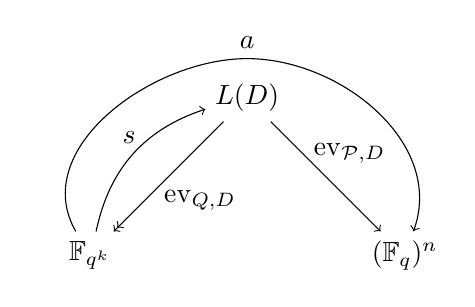
\begin{tikzpicture}
    \node (LD) at (2, 2) {$L(D)$};
    \node (Fqk) at (0, 0) {$\mathbb{F}_{q^k}$};
    \node (Fqn) at (4, 0) {$(\mathbb{F}_{q})^n$};
    \draw[->>] (LD) to (Fqk);
    \draw[->] (LD) to (Fqn);
    \draw[->] (Fqk) to[bend left] (LD);
    \node (s) at (0.5, 1.5) {$s$};
    \node (evQ) at (1.4, .7) {$\ev_{Q, D}$};
    \node (evP) at (3.3, 1.3) {$\ev_{\Pcal, D}$};
    \draw[->] (Fqk) to[out=120,in=180](2, 2.5) to[out=0, in=70] (Fqn);
    \node (a) at (2, 2.7) {$a$};
  \end{tikzpicture}
  \end{center}
  For all $1\leq i\leq n$, the map
  $x\mapsto f_x(P_i)$ is a linear form, so there exists an element
  $a_i\in\mathbb{F}_{q^k}$ such that
  \[
    \forall x\in\mathbb{F}_{q^k},\, f_x(P_i) = \ps{a_i}{x},
  \]
  thus
  \[
    \forall x\in\mathbb{F}_{q^k},\, a(x) = (\ps{a_1}{x}, \dots, \ps{a_n}{x}).
  \]
  Let $x, y, z\in\mathbb{F}_{q^k}$, and
  \[
    p = a(x)*a(y)*a(z)\in(\mathbb{F}_{q})^n
  \]
  be the coordinate-wise product of the elements $a(x)$, $a(y)$, and $a(z)$. In
  other words,
  \[
    p = (f_xf_yf_z(P_1), \dots, f_xf_yf_z(P_n)).
  \]
  Similarly, since the map $\ev_{\Pcal, 3D}$ is injective, it admits a left inverse $r$, \ie a
  map
  \[
        \begin{array}{cccc}
          r: & (\mathbb{F}_{q})^n & \to & L(D)
\end{array}
  \]
  such that
  \[
    r\circ\ev_{\Pcal, 3D} = \Id_{L(D)},
  \]
  where $\Id_{L(D)}$ is the identity map on $L(D)$. We
  also let
  \[
        \begin{array}{cccc}
          d: & (\mathbb{F}_{q})^n & \to & \mathbb{F}_{q^k} \\
\end{array}
  \]
  be the map $d = \ev_{Q, 3D}\circ r$.   The situation is sumed up in the
  following drawing.
  \begin{center}
  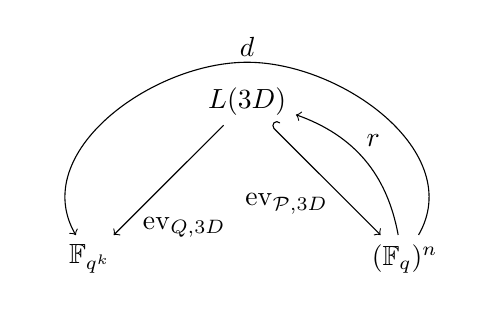
\begin{tikzpicture}
    \node (L3D) at (2, 2) {$L(3D)$};
    \node (Fqk) at (0, 0) {$\mathbb{F}_{q^k}$};
    \node (Fqn) at (4, 0) {$(\mathbb{F}_{q})^n$};
    \draw[right hook->] (L3D) to (Fqn);
    \draw[->] (L3D) to (Fqk);
    \draw[->] (Fqn) to[bend right] (L3D);
    \node (evP) at (2.5, .7) {$\ev_{\Pcal, 3D}$};
    \node (s) at (3.6, 1.5) {$r$};
    \node (evQ) at (1.2, .4) {$\ev_{Q, 3D}$};
    \draw[->] (Fqn) to[out=60,in=0](2, 2.5) to[out=180, in=120] (Fqk);
    \node (d) at (2, 2.7) {$d$};
  \end{tikzpicture}
\end{center}
The map $r$ is linear, so $d$ is also linear, by
  composition of two linear maps. Thus we have $n$ elements $d_1, \dots, d_n$ of
  $\mathbb{F}_{q^k}$ such that, for all $(x_1, \dots, x_n)\in\Img(\ev_{\Pcal,
  3D})$,
  \[
    d(x_1, \dots, x_n) = \sum_{i=1}^n x_i d_i.
  \]
Now
\[
  h = r(p)\in L(3D)
\]
is an element of $L(3D)$ such that
\[
  \forall 1\leq i\leq n,\,\ev_{\Pcal, 3D}(h) = f_xf_yf_z(P_i),
\]
but this is also the case for the function $f_xf_yf_z\in L(3D)$. Since the map
$\ev_{\Pcal, 3D}$ is injective, we have
\[
  h = f_xf_yf_z.
\]
Then, we have
\begin{equation*}
  \begin{split}
  d(p) &= \ev_{Q, 3D}(r(p))\\
  &= \ev_{Q, 3D}(h)\\
  &= h(Q)\\
  &= f_x(Q)f_y(Q)f_z(Q)\\
  &= s(x)(Q)s(y)(Q)s(z)(Q)\\
  &= \ev_{Q, D}\circ s(x)\ev_{Q, D}\circ s(y)\ev_{Q, D}\circ s(z)\\
  &= xyz.
  \end{split}
\end{equation*}
But we also have
\begin{equation*}
  \begin{split}
    p &= a(x)*a(y)*a(z)\\
    &= (\ps{a_1}{x}\ps{a_1}{y}\ps{a_1}{z}, \dots,
    \ps{a_n}{x}\ps{a_n}{y}\ps{a_n}{z}),
  \end{split}
\end{equation*}
so
\[
  d(p) = \sum_{i=1}^n\ps{a_i}{x}\ps{a_i}{y}\ps{a_i}{z}d_i
\]
and finally we have a $3$-symmetric decomposition of $m_3$:
\[
  xyz = \sum_{i=1}^n\ps{a_i}{x}\ps{a_i}{y}\ps{a_i}{z}d_i.
\]
\end{proof}
Now that we know the method to find $3$-symmetric decompositions of $m_3$, and thus
tri-symmetric decompositions of $m_2$, the question is, given $q$ and $k$, to
find an algebraic function field $F/\mathbb{F}_{q}$ satisfying
Proposition~\ref{prop:method}. If $F/\mathbb{F}_q$ is a function field of genus
$g$ and $G\in\D_F$ a divisor of $F$, Riemann's theorem states that
\[
  \dim L(G) \geq \deg G + 1 - g,
\]
with equality if $\deg G > 2g - 2$. Assume that there exist $Q\in\mathbb{P}_F$ a
place of $F$ of degree $k$, $P_1, \dots, P_n$ places of degree $1$ and
$D\in\D_F$ a divisor which support does not include $Q, P_1, \dots, P_n$. Since
\[
  \Ker(\ev_{\Pcal, 3D}:L(3D)\to(\mathbb{F}_{q})^n) = L(3D-P_1-\dots-P_n),
\]
the injectivity in Condition~\eqref{cond:2} is equivalent to
\[
  L(3D-P_1-\dots-P_n)=\left\{ 0 \right\}.
\]
This is the case if
\[
\deg(3D-P_1-\dots-P_n)<0,
\]
which is the case if
\[
  n > 3\deg D.
\]
Similarly, we have
\[
  \Ker(\ev_{Q, D}:L(D)\to\mathbb{F}_{q^k}) = L(D-Q),
\]
and the rank-nullity theorem states that
\[
  \dim L(D) = \dim\Ker(\ev_{Q, D})+\dim\Img(\ev_{Q, D}),
\]
so the surjectivity in Condition~\eqref{cond:1} is equivalent to
\[
  \dim L(D-Q) = \dim L(D) - k.
\]
A sufficient condition for the last equation to hold is that
\[
  \deg D > k+ 2g - 2,
\]
because
\begin{equation*}
  \begin{split}
  \deg(D-Q) &= \deg D - \deg Q\\
  &= \deg D - k\\
  &> 2g - 2
  \end{split}
\end{equation*}
and so
\begin{equation*}
  \begin{split}
    \dim L(D-Q) &= \deg(D-Q)+1-g\\
    &=\deg D+1-g-k\\
    &=\dim L(D)-k.
  \end{split}
\end{equation*}
Thus, a sufficient condition for Conditions~\eqref{cond:1} and~\eqref{cond:2} to
hold is that
\[
  \frac{n}{3} > \deg D > k + 2g - 2.
\]
If $\frac{n}{3}>k + 2g -1$, there exists an integer $\delta\in\mathbb{N}$ with
\[
  \frac{n}{3} > \delta > k +2g -2,
\]
\eg $\delta=k+2g-1$, therefore we can assume without loss of generality that there
exists a divisor $D$ of degree $\delta$ which support does not include $Q, P_1,
\dots, P_n$, thanks to the strong approximation theorem.

The remaining part is to prove that we can find suitable function fields for
each $q$ fixed and $k\to\infty$. It means that we look for a function field
$F/\mathbb{F}_q$ of genus $g$, with a place of degree $k$, and such that there
are at least $n$ places of degree $1$, with
\[
  n > 3k +6g - 3
\]
in order to apply Proposition~\ref{prop:method}. Let us start with the special case of $q\geq64$
a square. In this case, we know~\cite{STV92} that there exists a family of function fields
$F_i/\mathbb{F}_q$ of genus $g_i$ such that
\begin{enumerate}
  \item $g_i\to\infty$
  \item $\frac{g_{i+1}}{g_i}\to1$
  \item $N_i\sim (\sqrt q - 1)g_i$
\end{enumerate}
with
\[
  N_i = \Card\left\{ P\in\mathbb{P}_{F_i}\,|\,\deg P = 1 \right\}
\]
the number of places of degree $1$ of $F_i$. We also assume that the sequence
$(g_i)_i$ is increasing. For each $k$, let $g_{i(k)}$ be the
smallest genus $g_i$ such that
\[
  N_{i} > 3k + 6g_{i}.
\]
This is always possible to find such an index $i(k)$ since
\[
  N_i\sim (\sqrt q - 1)g_i
\]
and $\sqrt q -1 > 6$. By definition, we thus have
\[
  N_{i(k)-1}\leq 3k+6g_{i(k)-1}<3k+6g_{i(k)}<N_{i(k)}.
\]
Since $i(k)\to\infty$ when $k\to\infty$, we can use the asymptotic results on the
family of function fields $F_i$, so we know
\begin{equation*}
  \begin{split}
  N_{i(k)-1} &\sim (\sqrt q-1)g_{i(k)-1}\\
  &\sim (\sqrt q-1)g_{i(k)}\\
  &= (\sqrt q-1)g_{i(k)}+o(g_{i(k)}).
  \end{split}
\end{equation*}
Similarly,
\[
  N_{i(k)} = (\sqrt q -1)g_{i(k)}+o(g_{i(k)}),
\]
and so we deduce that
\begin{equation}
  3k = (\sqrt q -7)g_{i(k)} + o(g_{i(k)})
  \label{eqn:equivg}
\end{equation}
and
\begin{equation}
  g_{i(k)}= \frac{3}{\sqrt q - 7}k+o(k).
  \label{equivk}
\end{equation}
We know~\cite[Corollary 5.2.10.]{Stichtenoth09} there exists a place of degree
$k$ in $F_{i(k)}$ if we have
\begin{equation}
  2g_{i(k)} +1 \leq q^{(k-1)/2}(\sqrt q-1),
  \label{eqn:degreek}
\end{equation}
but thanks to Equation~\eqref{eqn:equivg} we know that
Inequation~\eqref{eqn:degreek} is true as soon as $k$ is large enough. Let
$k_0(q)$ be a constant such that~\eqref{eqn:degreek} is true for $k\geq k_0(q)$.
If $q\geq 64$ is a square and $k\geq k_0(q)$, we now know that we can find a
function field $F_{i(k)}$ in which Proposition~\ref{prop:method}
applies, so that we can find a $3$-symmetric decomposition of $m_3$ of length
$n$, and therefore a tri-symmetric decomposition $\mathbb{F}_{q^k}/\mathbb{F}_q$ of length $n$, with
\begin{equation*}
  \begin{split}
    n&\leq N_{i(k)}\\
    &= (\sqrt q -1)g_{i(k)}+o(g_{i(k)})\\
    &= \frac{\sqrt q -1}{\sqrt q -7}\cdot3\cdot k+o(k)\\
    &= O(k).
  \end{split}
\end{equation*}
We have thus proven that the tri-symmetric bilinear complexity of
$\mathbb{F}_{q^k}/F_{q}$ is \emph{linear} in $k$ for $q\geq64$ a square.

Let $q\geq3$ be a prime power, there exists an integer $d\in\mathbb{N}$ such that
\[
  q' = q^d \geq 64
\]
is a square. Let $\sym{q}{k}$ be the minimal length of a $3$-symmetric
decomposition of
\[
  m_3:\mathbb{F}_{q^{k}}\times\mathbb{F}_{q^k}\times\mathbb{F}_{q^k}\to\mathbb{F}_{q^k}.
\]
We know that there exists some constant
$N$ such that
\[
  \sym{q'}{k}\leq Nk
\]
for $k$ large enough, and since we know that

\[
  \sym{q}{kd}\leq\sym{q'}{k}\sym{q}{d},
\]
it follows that
\[
  \sym{q}{kd} \leq (sN)k.
\]
\begin{center}
  \begin{tikzpicture}
    \node (Fq) at (0, 0) {$\mathbb{F}_q$};
    \node (Fqk) at (-2, 2) {$\mathbb{F}_{q^k}$};
    \node (Fqd) at (2, 2) {$\mathbb{F}_{q'}$};
    \node (Fqkd) at (0, 4) {$\mathbb{F}_{q'^{k}}$};
    \draw (Fq) -- (Fqd);
    \draw (Fqd) -- (Fqkd);
    \draw (Fqk) -- (Fqkd);
    \draw (Fq) -- (Fqk);
    \node (s) at (1.2, .9) {$s$};
    \node (Ok) at (1.5, 3.1) {$N$};
  \end{tikzpicture}
\end{center}
Since
\[
  \mathbb{F}_{q^k}\subset\mathbb{F}_{q'^k}\cong\mathbb{F}_{q^{kd}},
\]
we also have
\begin{equation*}
  \begin{split}
    \sym{q}{k}&\leq\sym{q}{kd}\\
    &\leq (sN)k.
  \end{split}
\end{equation*}
Because $\tri{q}{k}\leq\sym{q}{k}$, it thus proves that the tri-symmetric bilinear complexity of
$\mathbb{F}_{q^k}/\mathbb{F}_q$ is asymptotically linear in $k$, for any $q\geq3$.

\bibliographystyle{plain}
\bibliography{erou}

\end{document}
